% A skeleton file for producing Computer Engineering reports
% https://kgcoe-git.rit.edu/jgm6496/KGCOEReport_template

\documentclass[CMPE]{KGCOEReport}

% The following should be changed to represent your personal information
\newcommand{\classCode}{CMPE 160}  % 4 char code with number
\newcommand{\name}{Andrei Tumbar}
\newcommand{\LabSectionNum}{4}
\newcommand{\LabInstructor}{Mr.\ Byers}	% The slash is to tell LaTeX that the period is between words
												% not sentences so it spaces correctly. It won't appear in the
												% final pdf
\newcommand{\TAs}{Sam Myers \\ Kobe Balin \\ Georgi Thomas}
\newcommand{\LectureSectionNum}{1}
\newcommand{\LectureInstructor}{Mr.\ Cliver}
\newcommand{\exerciseNumber}{7}
\newcommand{\exerciseDescription}{Sequential Circuit Elements}
\newcommand{\dateDone}{February 27th}
\newcommand{\dateSubmitted}{March 26th}

\graphicspath{{./lab7_media/}}

\usepackage{circuitikz}
\usepackage{tikz}
\usepackage{multirow}
\usepackage{titlesec}
\usepackage{float}
\usepackage{pgfplots, pgfplotstable}
\usepackage{lmodern}
\usepackage{siunitx}
\usepackage{subcaption}

\usepackage[usestackEOL]{stackengine}
\usepackage{scalerel}

\usepackage{kmap}
\usepackage[T1]{fontenc}

\usepackage{amsmath}

\def\lbar#1{\ThisStyle{%
  \setbox0=\hbox{$\SavedStyle#1$}%
  \stackengine{2.2\LMpt}{$\SavedStyle#1$}{\rule{\wd0}{0.1\LMpt}}{O}{c}{F}{F}{S}%
}}

\ctikzset{bipoles/not port/circle width=.4}
\ctikzset{tripoles/american xor port/height/.initial=.4}
\ctikzset{tripoles/american xor port/width/.initial=.6}

\DeclareFontFamily{U}{mathx}{\hyphenchar\font45}
\DeclareFontShape{U}{mathx}{m}{n}{ <-> mathx10 }{}
\DeclareSymbolFont{mathx}{U}{mathx}{m}{n}
\DeclareFontSubstitution{U}{mathx}{m}{n}
\DeclareMathAccent{\widebar}{\mathalpha}{mathx}{"73}

\makeatletter
\newcommand{\cwidebar}[2][0]{{\mathpalette\@cwidebar{{#1}{#2}}}}
\newcommand{\@cwidebar}[2]{\@cwideb@r{#1}#2}
\newcommand{\@cwideb@r}[3]{%
  \sbox\z@{$\m@th\mkern-#2mu#3\mkern#2mu$}%
  \widebar{\box\z@}%
}
\makeatother

\begin{document}
\maketitle

\section*{Abstract}
In this laboratory exercise a D flip-flop was created using two D-latches. This circuit configuration allows the resultant output value to only change on a clock edge. By implementing two D-latches with active-low enable, they were connected together to create the D flip-flop. Modelsim was used to simulate the design created in Quartus. Finally, the circuit was implemented on a breadboard and the clock signal was created using a $1\,Hz$ wave generator.

\section*{Design Methodology}

A D-latch is a circuit that can store boolean values and load new values. For this functionality, three actions must be implemented. \texttt{SET}, \texttt{RESET}, and \texttt{HOLD} are needed. \texttt{SET} and \texttt{RESET} are used to load the value 1 or 0 into the latch. \texttt{HOLD} will keep the previous value constant.

\begin{table}[h!]
\renewcommand{\arraystretch}{1.2}
\setlength{\tabcolsep}{12pt}
\caption{Function table for low enable D-latch}
\begin{center}
\begin{tabular}{|c|c||c|c|}
\hline
En & D & Q & Qn\\\hline
0 & 0 & 0 & 1\\\hline
0 & 1 & 1 & 0\\\hline
1 & X & $Q_0$ & $\widebar{Q_0}$\\\hline

\end{tabular}
\end{center}
\label{tab:dlatch}
\end{table}

Table \ref{tab:dlatch} shows the latch with a two input function. Because this D-latch is active-low enable, when the enable signal is low, Q takes on the value of D. When the enable is high, Q keeps the old value. This latch is asynchronous meaning that the Q value will change immediatly if the enable is low.

\begin{figure}[h!]
	\centering
	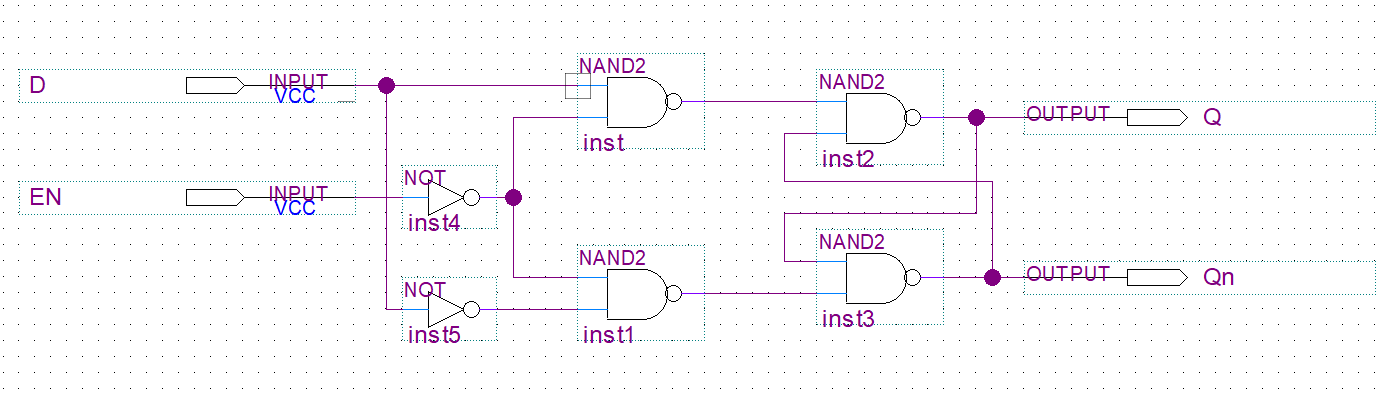
\includegraphics[width=\textwidth]{schematic1}
	\caption{D-latch circuit schematic}
	\label{fig:dlatch-schem}
\end{figure}

Figure \ref{fig:dlatch-schem} is a circuit schematic of the two-input D-latch described in Table \ref{tab:dlatch}. There is an inverter placed after the enable input to cause the latch to be active low.

To create a clock sensitive and synchronous D flip-flop, two D-latches must be used. By using two latches and inverting the enable signal used on the second one, the time delay between the two enables will cause the resultant value to only change on a clock edge.

\begin{table}[h!]
\renewcommand{\arraystretch}{1.2}
\setlength{\tabcolsep}{12pt}
\caption{Rising edge-triggered D flip-flop}
\begin{center}
\begin{tabular}{|c|c||c|c|}
\hline
clk & D & Q & Qn\\\hline
$\uparrow$ & 0 & 0 & 1\\\hline
$\uparrow$ & 1 & 1 & 0\\\hline
otherwise  & X & $Q_0$ & $\widebar{Q_0}$\\\hline

\end{tabular}
\end{center}
\label{tab:dflipflop}
\end{table}

Table \ref{tab:dflipflop} is very similar to Table \ref{tab:dlatch} in that the resultant values of Q and Qn are the same. However, Q only changes on a rising edge of the enable/clock signal.

\begin{figure}[h!]
	\centering
	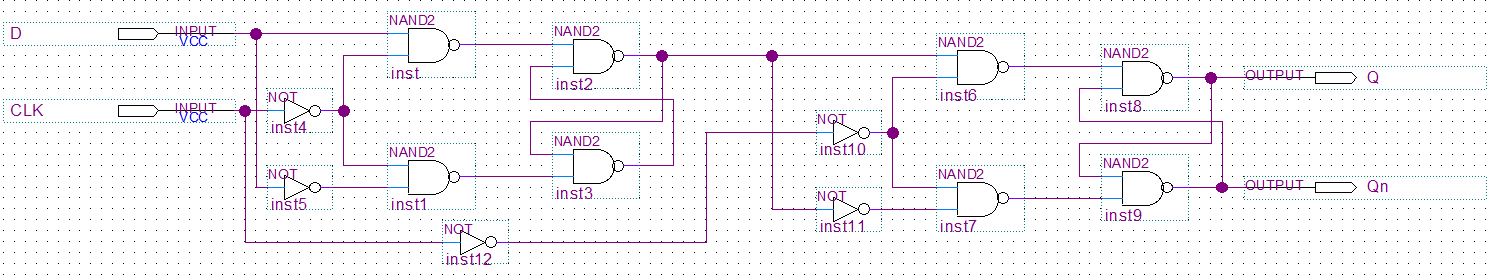
\includegraphics[width=\textwidth]{schematic2}
	\caption{D flip-flop circuit schematic}
	\label{fig:dflipflop-schem}
\end{figure}

Figure \ref{fig:dflipflop-schem} shows the circuit configuration of the D flip-flop using two D-latches. The output of the first latch is sent to the input of the second latch. The \texttt{CLK} signal is inverted and sent to the enable of the second D-latch. The time delay on the inverter of the \texttt{CLK} will cause the output, Q, to change only when the clock value is rising.

\section*{Results and Analysis}

After the D-latch and flip-flop were designed in Quartus, a simulation in Modelsim was performed.

\begin{figure}[h!]
	\centering
	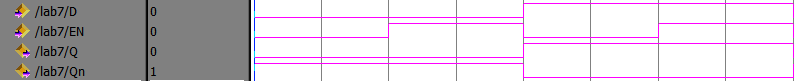
\includegraphics[width=\textwidth]{part1}
	\caption{D-latch simulation}
	\label{fig:dlatch-sim}
\end{figure}

Figure \ref{fig:dlatch-sim} shows the results of the a modelsim simulation run with the D-latch circuit. When the \texttt{EN} signal was low, \texttt{Q} took the value of \texttt{D}. When the \texttt{EN} is high, \texttt{D} is ignored and \texttt{Q} is held to the current value. This is exactly how the D-latch was described in the previous section.\\

The D flip-flop was also simulated in this exercise. The enable signal however was changed to a clock signal.\pagebreak

\begin{figure}[h!]
	\centering
	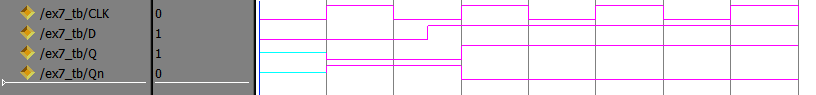
\includegraphics[width=\textwidth]{part2}
	\caption{D flip-flop simulation}
	\label{fig:dflipflop-sim}
\end{figure}

The change on the D signal in Figure \ref{fig:dflipflop-sim} was placed offset to the \texttt{CLK} changes as to show a typical occurance in this circuit. Also, if the input signal, \texttt{D} were to change too closely to the clock edge, the circuit would enter a metastasis in which either 0 or 1 could result. The results of this simulation were as expected. The value of \texttt{Q} is unknown before the first clock edge therefore depicted with a line inbetween the logical 1 and 0 values. On every rising clock edge \texttt{Q} takes on the value of \texttt{D}.

\section*{Conclusion}

This exercise was implemented a full adder using simple logic gates. Then a 4-bit adder to create an adder/subtractor with 9-inputs and 5-outputs. A simulation of the full adder was performed in Multisim to verify the circuit against a Karnaugh Map. Both the full adder and the 4-bit adder/subtractor were constructed on a breadboard to test the signal outputs using LEDs. The exercise was successful in that the correct outputs were displayed given arbitrary inputs.




\section*{Questions}

\begin{enumerate}
  \item The simplest way to combine two full adders is to wire the $C_{out}$ of the LSB to the $C_{in}$ of the MSB.
  
\begin{figure}[htbp]
	\begin{center}
		\begin{circuitikz}
		
		\draw (0,0) node[dipchip,
			num pins=6,
			hide numbers, no topmark, external pins width=0.0](LSB){A0};
	
		\node [right, font=\tiny] at (LSB.bpin 1) {A0};
		\node [right, font=\tiny] at (LSB.bpin 2) {B0};
		\node [right, font=\tiny] at (LSB.bpin 3) {$C_{in}$};
		\node [left, font=\tiny]  at (LSB.bpin 6) {Sum};
		\node [left, font=\tiny]  at (LSB.bpin 4) {$C_{out}$};
		
		\draw (3,0) node[dipchip,
			num pins=6,
			hide numbers, no topmark, external pins width=0.0](MSB){A1};
	
		\node [right, font=\tiny] at (MSB.bpin 1) {A1};
		\node [right, font=\tiny] at (MSB.bpin 2) {B1};
		\node [right, font=\tiny] at (MSB.bpin 3) {$C_{in}$};
		\node [left, font=\tiny]  at (MSB.bpin 6) {Sum};
		\node [left, font=\tiny]  at (MSB.bpin 4) {$C_{out}$};
		
		\coordinate (start) at (0,-2);
		
		\draw (start) ++(0,0) coordinate(A0) node [below, font=\tiny]{A0};
		\draw (start) ++(1,0) coordinate(B0) node [below, font=\tiny]{B0};
		\draw (start) ++(2,0) coordinate(A1) node [below, font=\tiny]{A1};
		\draw (start) ++(3,0) coordinate(B1) node [below, font=\tiny]{B1};
		
		\draw (A0) |- ++(-1.5,0.5) |- (LSB.pin 1);
		\draw (B0) |- ++(-2.25,0.75) |- (LSB.pin 2);
		\draw (A1) |- ++(-0.5, 0.5) |- (MSB.pin 1);
		\draw (B1) |- ++(-1.25,0.75) |- (MSB.pin 2);
		
		\draw (LSB.pin 4) -- (MSB.pin 3);
		\draw (LSB.pin 6) -| ++(0.5,1) node[above, font=\tiny]{S0};
		\draw (MSB.pin 6) -| ++(0.5,1) node[above, font=\tiny]{S1};
		
		\draw (LSB.pin 3) -- ++(-1.5,0) node[ground]{};
		\draw (MSB.pin 4) -- ++(0.5,0) node[right, font=\tiny]{$C_{out}$};
		
		\end{circuitikz}
	\end{center}
	\caption{Two bit ripple-carry adder.}
	\label{fig:ripple}
\end{figure}

Figure \ref{fig:ripple} shows two full adders chained together by feeding the $C_{out}$ of the first into the $C_{in}$ of the second. The $C_{in}$ of the LSB is connected to ground or 0 because there is no previous bit to carry from.

  \item Overflow can be detected in an adder by analysing the signs of the inputs and output. If the signs of the inputs are opposite, there is no chance for overflow because the output is closer to zero relative to the inputs. An overflow occurs when the signs of the inputs are different from that of the output. For example in a 3-bit binary number, $1 + 7 = -8$. The inputs are both positive however the output is negative therefore an overflow occured. A boolean expression can be used to define this behavior. Given $A_N$ and $B_N$ being the N\textsuperscript{th} bit in an N-bit binary number as inputs and $F_N$ the N\textsuperscript{th} bit in the output, the following expression can be derived to define $F_{overflow}$.

\begin{equation}
\label{eq:overflow}
F_{overflow} = (AB + \widebar{A_N}\widebar{B_N}) \cdot (A_N \oplus F) = \lbar{A_N \oplus B_N} \cdot (A_N \oplus F_N)
\end{equation} 

Equation \ref{eq:overflow} shows two implementations using a XNOR gate and an XOR gate or and XOR gate and the constituants of the XNOR. The first compontent checks if the signs of the inputs are the same, the second portion checks if that sign is different from the sign of the output. If both of those conditions meet, an overflow occured.

  \item The circuit from Part 2 produces incorrect answers in some of the test cases because an overflow occured. Because the number is 2's comparison, the first bit acts as the sign and therefore a number may not exceed over 7 or under -8. When a sum of two numbers goes beyond the range described, the number will loop around to the other extreme.
  
  \item If the result was extended to use a fifth bit, the answer would not be completely correct. The carry out of the four-bit adder needs to be added to the fifth bit of the augend and addend. However if the sign of the two operands are same, the result of the carry out bit can be used. To fix this, if the signs of the operands are different, the value of the fifth bit is the inverse of the carry out. If the operands are the same, the carry out may be used as the fifth bit. This can be defined using the following expression.

\begin{equation}
F_{N+1} = (A_N \oplus B_N) \oplus C_N
\end{equation}

If the sign of $A$ and $B$ are different the first XOR gate will be 1. If this output is 1, the second XOR gate will act as an inverter. If they are equal, the second XOR will act as a wire.
  
  \item Design a 4-bit adder/subtractor so that the overall circuit will produce a 5-bit result that is always correct in the case of overflow.

\begin{figure}[htbp]
	\begin{center}
		\begin{circuitikz}
		
		\coordinate (SS) at (-2,-3);
		\draw (SS) ++(0,3) coordinate (AS);
		\coordinate (BS) at (SS);
		
		\draw (AS) ++(0,0)   coordinate(A3) node [left, font=\tiny]{A3};
		\draw (AS) ++(0,0.5) coordinate(A2) node [left, font=\tiny]{A2};
		\draw (AS) ++(0,1)   coordinate(A1) node [left, font=\tiny]{A1};
		\draw (AS) ++(0,1.5) coordinate(A0) node [left, font=\tiny]{A0};
		
		\draw (BS) ++(0,0)    coordinate(B3) node [left, font=\tiny]{B3};
		\draw (BS) ++(0,0.75) coordinate(B2) node [left, font=\tiny]{B2};
		\draw (BS) ++(0,1.5)  coordinate(B1) node [left, font=\tiny]{B1};
		\draw (BS) ++(0,2.25) coordinate(B0) node [left, font=\tiny]{B0};
		
		\draw (SS) ++(0,-1) coordinate(CIN) node [left, font=\tiny]{Control};
		
		\draw (A0) ++(4,-.20) node[dipchip,
			num pins=20,
			hide numbers, no topmark, external pins width=0.0, anchor=pin 3](ADD){}
			
			(ADD.center)
			
			node[label, rotate=-90]{74LS83}
			;
	
		\node [right, font=\tiny] at (ADD.bpin 1) {C0} ;
		\node [right, font=\tiny] at (ADD.bpin 3) {A0};
		\node [right, font=\tiny] at (ADD.bpin 4) {B0};
		\node [right, font=\tiny] at (ADD.bpin 5) {A1};
		\node [right, font=\tiny] at (ADD.bpin 6) {B1};
		\node [right, font=\tiny] at (ADD.bpin 7) {A2};
		\node [right, font=\tiny] at (ADD.bpin 8) {B2};
		\node [right, font=\tiny] at (ADD.bpin 9) {A3};
		\node [right, font=\tiny] at (ADD.bpin 10) {B3};
		
		\coordinate (IC0) at (ADD.pin 1);
		\coordinate (IA0) at (ADD.pin 3);
		\coordinate (IB0) at (ADD.pin 4);
		\coordinate (IA1) at (ADD.pin 5);
		\coordinate (IB1) at (ADD.pin 6);
		\coordinate (IA2) at (ADD.pin 7);
		\coordinate (IB2) at (ADD.pin 8);
		\coordinate (IA3) at (ADD.pin 9);
		\coordinate (IB3) at (ADD.pin 10);
		
		\node [left, font=\tiny]  at (ADD.bpin 13) {C3};
		\node [left, font=\tiny]  at (ADD.bpin 15) {S3};
		\node [left, font=\tiny]  at (ADD.bpin 16) {S2};
		\node [left, font=\tiny]  at (ADD.bpin 17) {S1};
		\node [left, font=\tiny]  at (ADD.bpin 18) {S0};
		
		\coordinate (OC3) at (ADD.pin 13);
		\coordinate (OS0) at (ADD.pin 18);
		\coordinate (OS1) at (ADD.pin 17);
		\coordinate (OS2) at (ADD.pin 16);
		\coordinate (OS3) at (ADD.pin 15);
		
		\draw (B0) ++(0.5,0) node[xor port, anchor=in 1] (xor0) {};
		\draw (B1) ++(0.5,0) node[xor port, anchor=in 1] (xor1) {};
		\draw (B2) ++(0.5,0) node[xor port, anchor=in 1] (xor2) {};
		\draw (B3) ++(0.5,0) node[xor port, anchor=in 1] (xor3) {};
		
		\draw (B0) -- (xor0.in 1)
			  (B1) -- (xor1.in 1)
			  (B2) -- (xor2.in 1)
			  (B3) -- (xor3.in 1)
		;
		
		\draw (xor3.in 2) to [short, -*] ++(-.125,0) coordinate(c3) |- (CIN);
		\draw (xor2.in 2) to [short, -*] ++(-.125,0) coordinate(c2) |- (c3);
		\draw (xor1.in 2) to [short, -*] ++(-.125,0) coordinate(c1) |- (c2);
		\draw (xor0.in 2) to [short, -*] ++(-.125,0) coordinate(c0) |- (c1);
		\draw (c0) |- (IC0);
		
		\draw (A3) -| ([xshift=-6mm]IA3) coordinate(a3c) to[short, *-] (IA3);
		\draw (A2) -| ([xshift=-4mm]IA2) -- (IA2);
		\draw (A1) -| ([xshift=-2mm]IA1) -- (IA1);
		\draw (A0) -| ([xshift=-1mm]IA0) -- (IA0);
		
		\draw (xor0.out) -- ++(0.25,0) |- (IB0);
		\draw (xor1.out) -- ++(0.5, 0) |- (IB1);
		\draw (xor2.out) -- ++(0.75,0) |- (IB2);
		\draw (xor3.out) to[short,-*] ++(1,0) coordinate(b3c) (b3c) |- (IB3);
		
		\draw (IB3) ++(1.25,-1) node[xor port] (xor_o1){};
		\draw (b3c) |- (xor_o1.in 2);
		\draw (a3c) |- (xor_o1.in 1);
		
		\draw (OS0) -- ++(1,0) node[right, font=\tiny]{F0};
		\draw (OS1) -- ++(1,0) node[right, font=\tiny]{F1};
		\draw (OS2) -- ++(1,0) node[right, font=\tiny]{F2};
		\draw (OS3) -- ++(1,0) node[right, font=\tiny]{F3};
		
		\draw (OC3) -- ++(0.25,0) node[xor port, anchor=in 1](xor_o2){};
		\draw (xor_o1.out) -| ([xshift=-1mm]xor_o2.in 2) -- (xor_o2.in 2);
		\draw (xor_o2.out) -- ++(0.25,0) node[right, font=\tiny]{F4};
		
		\end{circuitikz}
	\end{center}
	\caption{4-bit adder/subtractor with 5-bit output.}
	\label{fig:overflow_adder}
\end{figure}

\end{enumerate}

\end{document}
